\documentclass[11pt]{article}
\usepackage[czech]{babel}
\usepackage[utf8]{inputenc}
\usepackage[T1]{fontenc}
\usepackage{xcolor}
\usepackage{listings}
\usepackage{indentfirst}
\usepackage{amsmath}
\usepackage{amssymb}
\usepackage{hyperref}
\usepackage{graphicx}
\usepackage{float}
\usepackage{mathtools}
\usepackage[hyphenbreaks]{breakurl}
\DeclarePairedDelimiter{\abs}{\lvert}{\rvert}
\graphicspath{ {./images/} }

\definecolor{codegreen}{rgb}{0,0.6,0}
\definecolor{codegray}{rgb}{0.5,0.5,0.5}
\definecolor{codepurple}{rgb}{0.58,0,0.82}
\definecolor{backcolour}{rgb}{0.95,0.95,0.92}

\lstdefinestyle{mystyle}{
    backgroundcolor=\color{backcolour},   
    commentstyle=\color{codegreen},
    keywordstyle=\color{magenta},
    numberstyle=\tiny\color{codegray},
    stringstyle=\color{codepurple},
    basicstyle=\ttfamily\footnotesize,
    breakatwhitespace=false,         
    breaklines=true,                 
    captionpos=b,                    
    keepspaces=true,                 
    numbers=left,                    
    numbersep=5pt,                  
    showspaces=false,                
    showstringspaces=false,
    showtabs=false,                  
    tabsize=2
}

\lstset{style=mystyle}

\title{Dlouhodobá maturitní práce \\
\large Teoreticky rozebrat a popsat shorův kvantový algoritmus na lámání šifry RSA. 
Implementovat algoritmus v nějakém simulátoru a použít ho na prolomení RSA s malým modulusem}

\author{Dmitry Leshchinskiy}
\date{\today}

\makeatletter
\let\mytitle\@title
\let\myauthor\@author
\let\mydate\@date
\makeatother

\begin{document}
\maketitle
\newpage

\tableofcontents
\newpage

\section{Úvod}
Cílem mé práce je vytvořit funkční simulátor kvantového počítače, na kterém bych zkusil implementovat Shorův algoritmus, který by se dal využít pro prolomení RSA.
\par Nejdřív popíšu, co je to RSA.
V teto sekci vysvětlím, jak se dopočítávají kliče pro šifrovaní a dešifrovaní a jak je využít pro zašifrovaní zprávy.
\par V další kapitole popišu matematický model kvantového počítače.
Vysvětlím, co je to qubit a jak se značí.
Na příkladech předvedu funkčnost některých kvantových hradel.
\par Následující kapitola se zabývá popisem mé knihovny, kterou jsem vytvořil pravě pro účel seznámeni s kvantovými počítači.
Obsahuje popis dostupných funkci pro tvorbu a simulaci kvantových algoritmu.
\par Další kapitola primo navazuje na předchozí.
Zde ukážu, jak lze pomoci mé knihovny vytvořit a simulovat kvantové obvody.
\par Na závěr teoreticky popisu Shorův algoritmus a předvedu kód pomoci, kterého se mi povedlo tento algoritmus nasimulovat.
\newpage

\section{Čestné prohlášení}
Prohlašuji, že jsem předkládanou dlouhodobou maturitní práci vypracoval
sám a uvedl jsem veškerou použitou literaturu a bibliografické citace.
\\ \\ \\
\par V Praze dne: \mydate \\
\par \myauthor: \hrulefill
\newpage

\section{Úvod do RSA}
\subsection{Co je to RSA?}

RSA je asymetrická šifra s otevřeným klíčem, která byla veřejně publikovaná v roce 1977.
Stvořili ji 3 lidi: Ron Rivest, Adi Shamir a Leonard Adleman.
Asymetrické šifry jsou ty, které pro šifrovaní a dešifrovaní využívají dvojici klíčů.
Využívá jednosměrnou funkci, která znemožňuje použiti stejného klíče pro šifrovaní a dešifrovaní.
Pro použiti teto šifry je potřeba si vypočítat otevřeny klíč, kterým se bude šifrovat zprava určena pro vás, a privátní klíč, kterým vy budete šifru dešifrovat.
K aktuálnímu dni se tato šifra povazuje za bezpečnou.

\subsection{Princip RSA}
Když budu chtít někomu poslat zakódovanou zprávu pomoci RSA, potřebuji si od adresáta dostat jeho veřejný klíč.
Tímto klíčem si zakóduji zprávu a odešlu.
Příjemce až zprávu dostane, dešifruje ji pomoci svého privátního klíče.
\par Bezpečnost RSA je postavena na předpokladu, že je výpočetně dost náročné faktorizovat číslo.
Faktorizovat číslo znamená rozložit jej na součin prvočísel.

\subsection{Výpočet klíčů teorie}
Nejdřív se vybírá dvojice prvočísel: $p, q$.
Následně se vypočítá jejich násobek. Označíme ho za $N$.
Dále si nadefinujeme $\varphi (N)$ jako $(p - 1) \cdot (q - 1)$.
\par V následujícím kroku se musí vybrat číslo $e$, pro které platí, že je nesoudělné s $\varphi (N)$.
Pro nalezeni $e$ lze využít rozšířeny Euklidův algoritmus.
Z praktického hlediska se číslo $e$ vybírá tak, aby obsahovalo malý počet bitu rovných $1$.
To je z důvodu rychlejšího šifrovaní, které se provádí pomoci umocňovaní.
Posledním krokem je určit číslo $d$, což lze v praxi nalézt rozšířeným Euklidovým algoritmem.
Pro d platí:
$$ ed \bmod \varphi (N) = 1 $$
Veřejný klíč je pak dvojice: $e, N$ \\
Privátní klíč je pak dvojice: $d, N$

\subsection{Výpočet klíčů ukázka}
\noindent Zvolíme si nejprve $p, q$:
$$p = 83, q = 89$$
Spočítám $N, \varphi (N)$:
$$N = pq = 83 \cdot 89 = 7387$$
$$\varphi (N) = (p - 1)(q - 1) = 82 \cdot 88 = 7216$$
Získám $e, d$:
$$e = 3 \because gcd(e, \varphi (N)) = 1$$
$$d = 4811 \because ed \bmod \varphi (N) = 1$$
Poskládám klíče:
Veřejný: $(3, 7387)$
Privátní: $(4811, 7387)$

\subsection{Šifrovaní a dešifrovaní}
Nejdřív si popišem šifrovaní.
Mějme zprávu $m$ a veřejný klíč $(e, N)$.
Pak se zprava zašifruje do $c$ následovně:
$$c = m^e \bmod N$$
\par Proto abychom mohli zprávy dešifrovat, potřebujeme privátní klíč.
Pak se zprava $c$ dešifruje pomoci privátního klíče $(d, N)$ do $m$ následně:
$$m = c^d \bmod N$$
\par Všimneme si, že může docházet k umocnění velkým exponentem.
Tento výpočet by mohl trvat dost dlouho a zároveň by se spotřebovalo víc paměti pro velká čísla.
Proto v praxi se využívá úspornější metoda, která využívá rovnost:
$$(a * b) \bmod N = ((a \bmod N)(b \bmod N)) \bmod N$$
Tedy můžeme modulit po každém násobeni.
Však počet iteraci násobeni bude roven hodnotě exponentu.
Pro jejich zmenšeni lze využít binární umocňovaní.
Během teto metody umocňovaní, procházíme pobitově exponent od nejvyššího bitu.
Když je bit roven 0, pak umocníme druhou mocninou poslední mezi výsledek.
Jestliže je bit roven 1, pak umocníme druhou mocninou poslední mezi výsledek a vynásobíme původním základem\footnote{\url{https://en.wikipedia.org/wiki/Exponentiation_by_squaring}}.

\subsection{Prolomeni RSA}
Jak již bylo zmíněno, RSA se povazuje za bezpečnou šifru.
Na venek je přístupna jen zašifrovaná zprava $c$ a veřejný klíč $(e, N)$, kterým byla zprava zašifrovaná.

\par Pro dešifrovaní potřebujme privátní klíč $(d, N)$.
Pro výpočet $d$ potřebujeme si dopočítat $\varphi (N)$, který se počítá z $p$ a $q$.
Naštěstí nebo k neštěstí, záleží na pohledu, známe $N$, což je součin $p$ a $q$.
Takže potřebujeme jen rozložit $N$ na součin dvou prvočísel neboli faktorizovat.

\par Zatím neexistuje žádný algoritmus pro faktorizaci, který by běžel na klasickém počítací v polynomiálním čase.
Avšak v roce 1994 se podařilo P. Shorovi, americkému profesorovi matematiky v MIT, vymyslet algoritmus, který by běžel částečné na kvantovém počítací, a výsledkem je rozložené číslo na součin prvočísel.
Ten algoritmus si pojmenoval jako Shorův algoritmus\footnote{\url{https://arxiv.org/pdf/quant-ph/9508027.pdf}}.

\newpage

\section{Úvod do Kvantových počítačů}
\subsection{Co je kvantový počítač?}
Kvantový počítač je teoreticky model zařízeni pro výpočty.
Primo využívá fenomény z kvantové mechaniky jako superpozice nebo interference.
Zatím co klasicky počítač operuje s bity, kvantový počítač operuje s qubity.
Jednotlivým skupinám qubitu se říká registr.

\subsection{Co je to Qubit?}
Klasicky bit v počítací může nabývat hodnot ${0, 1}$.
Qubit může byt $0$, $1$ nebo kombinaci obou.
Matematicky ho modelujeme jako dvourozměrný komplexní vektor:
$$|q\rangle = \alpha|0\rangle + \beta|1\rangle$$
\par kde $\alpha,\beta\in\mathbb{C}$ jsou koeficienty, které určují pravděpodobnost změřeni qubitu ve stavu $0$ nebo $1$.
Součet druhých mocnin koeficientu se musí rovnat $1$:
$$\alpha^2 + \beta^2 = 1$$
\par Zápis $|0\rangle$ a $|1\rangle$ není nic jiného než jenom zkráceny zápis vektoru.
Můžeme je rozepsat takto:
$$|0\rangle = \begin{bmatrix}
        1 \\
        0
    \end{bmatrix} |1\rangle = \begin{bmatrix}
        0 \\
        1
    \end{bmatrix}  $$
\par Upravíme a přepíšeme stav qubitu $|q\rangle$ jako:
$$|q\rangle = \begin{bmatrix}
        \alpha \\
        \beta
    \end{bmatrix}$$

\par Kvantový počítač by byl k ničemu, pokud by neslo získat výsledek z výpočtu.
Za výsledek se povazuje jeden konkrétní stav kvantového počítače z množiny možných stavu pro konkrétní algoritmus.
Pro některé stavy je pravděpodobnost výskytu větší než u jiných.
Abychom dostali výsledek z reálného kvantového počítače, se používá měřeni.
Podstatnou vlastnosti měřeni je, že qubity že stavu superpozice se dostanou do stavu $|0\rangle$ nebo $|1\rangle$.
Ukážeme si, jak matematicky funguje měřeni.
Proto abychom zjistili pravděpodobnost pro konkrétní stav, nám stačí umocnit na druhou násobek transponovaného vektoru hledaného stavu a vektoru $|q\rangle$:
$$|\langle 0 | q \rangle|^2 = \abs*{\begin{bmatrix}
            1 & 0
        \end{bmatrix}\begin{bmatrix}
            \alpha \\
            \beta
        \end{bmatrix}}^2 = \alpha ^ 2$$

$$|\langle 1 | q \rangle|^2 = \abs*{\begin{bmatrix}
            0 & 1
        \end{bmatrix}\begin{bmatrix}
            \alpha \\
            \beta
        \end{bmatrix}}^2 = \beta ^ 2$$

\subsection{Blochova koule}
Blochova koule se často využívá pro vizualizaci jednoho qubitu.
Qubit je reprezentován libovolným bodem na kouli.
Severní pól koule odpovídá stavu $|0\rangle$, zatímco jižní pól odpovídá stavu $|1\rangle$.
\sloppy
Vizualizace může vypadat takhle\footnote{\url{https://qubits.cz/serialy/kvantovy-serial-dil-2-kvantove-pocitace-qubit/}}:
\begin{figure}[H]
    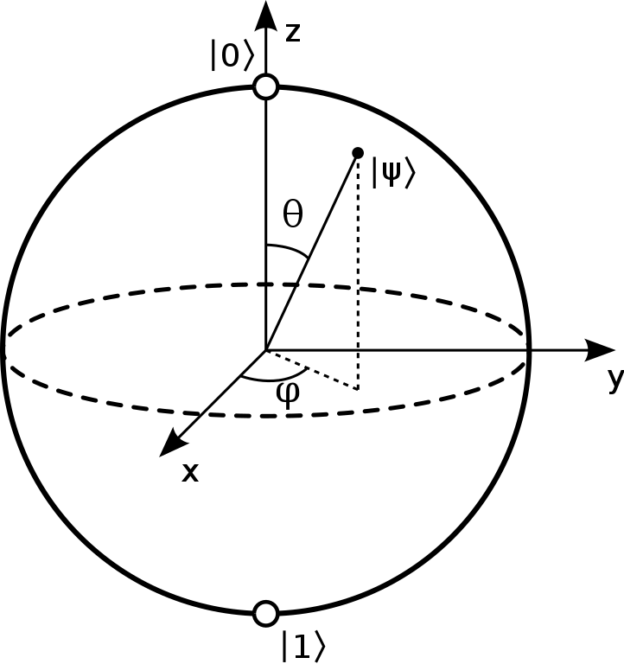
\includegraphics[scale=0.25]{Bloch_sphere}
    \centering
\end{figure}

\par Drive jsem definoval stav qubitu pomoci $\alpha$ a $\beta$.
Lze taky definovat stav qubitu pomoci dvou uhlu $\varphi$ a $\theta$:
$$|q\rangle = \cos{\frac{\theta}{2}}|0\rangle + e^{i\varphi}\sin{\frac{\theta}{2}}|1\rangle $$

\subsection{Registr Qubitu}
Ve výpočtech většinou nebudeme pracovat s jedným qubitem ale s celým registrem qubitu. Zkráceny zápis by vypadal takto:
$$|001\rangle$$
\par To znamená, že mam 3 qubity, první 2 jsou nastavené na 0, poslední je nastaven na 1.
Registr o $n$ bitech se matematicky modeluje jako $2^n$-rozměrný vektor. Kombinace jednotlivých qubitů do celého registru lze formálně provést operací Kroneckerova součinu, například takto:
$$|q\rangle = |001\rangle = |0\rangle \otimes |0\rangle \otimes |1\rangle = \begin{bmatrix}
        0 \\
        1 \\
        0 \\
        0 \\
        0 \\
        0 \\
        0 \\
        0 \\
    \end{bmatrix}$$
\par Pravidla pro měřeni funguji stejně:
$$|\langle001|q\rangle|^2 = 1$$
$$|\langle 011|q\rangle|^2 = 0$$

\subsection{Kvantové hradlo}
V booleve algebře máme logická hradla typu OR, AND, XOR.
To jsou hradla, které dostávají vstup bitu a produkuji vystup.
Základní operace s kvantovými registry můžeme provádět jistou analogií – kvantovými hradly.
Největší rozdíl je v tom, že kvantová hradla provádí jenom reverzibilní operace.
Všechna kvantová hradla jsou reverzibilní.
To znamená, že ke každému hradlu existuje jeho inverzní hradlo, které když aplikujeme po sobě tak celý obvod bude zachovávat stav registru.
\par Každé hradlo je matematicky definováno čtvercovou matici o rozměrech $2^n \times 2^n$, kde $n$ je počet qubitu.
Pro aplikovaní hradla je potřeba vynásobit mezi sebou matici hradla a vektor stavu $|q\rangle$.
\par Základní kvantové hradlo je \textbf{I} jako identita.
Přesněji řečeno nemění stav vektoru a výstupní qubit se tedy vždy rovná vstupnímu. I tak bude potřeba pro některé výpočty.
Její matice vypadá takto:
$$I = \begin{bmatrix}
        1 & 0 \\
        0 & 1
    \end{bmatrix}$$
\par Nejjednodušší reverzibilní hradlo v klasickém počítací je NOT.
Provádí negaci bitu. V kvantovém světě existuje podobné hradlo, které také neguje hodnotu.
Přesněji řečeno otáčí Blochovou kouli podle $x$ osy o $\pi$ radiánu. Značí se jako \textbf{X} gate.
Jeho matice je následující:
$$X = \begin{bmatrix}
        0 & 1 \\
        1 & 0
    \end{bmatrix}$$
\par Jako důkaz, že se jedná o hradlo reverzibilní, mužem zkusit je poskládat za sebou a podívat se co nám vyjde.
To znamená, že jejich matice vynásobíme mezi sebou:
$$XX = \begin{bmatrix}
        0 & 1 \\
        1 & 0
    \end{bmatrix}\begin{bmatrix}
        0 & 1 \\
        1 & 0
    \end{bmatrix} = \begin{bmatrix}
        1 & 0 \\
        0 & 1
    \end{bmatrix} = I$$

\par Ve výsledku máme hradlo \textbf{I}, které jak víme neděla nic s vektorem stavu $|q\rangle$.
\par Dalším hodně zajímavým hradlem, který bude potřeba pro Shorův algoritmus je Hadamard gate, který se značí \textbf{H}. Jeho matice:
$$H = \frac{1}{\sqrt{2}}\begin{bmatrix}
        1 & 1  \\
        1 & -1
    \end{bmatrix}$$
\par Toto hradlo převádí qubit do stavu superpozice. Důležité je zmínit, že superpozice vytvořena z qubitu ve stavu 0, se bude výrazně lišit od superpozice vytvořené z qubitu ve stavu 1.
Tady je výpočet:
$$H|0\rangle = \frac{1}{\sqrt{2}}\begin{bmatrix}
        1 & 1  \\
        1 & -1
    \end{bmatrix}\begin{bmatrix}
        1 \\
        0
    \end{bmatrix} = \frac{1}{\sqrt{2}}\begin{bmatrix}
        1 \\
        1
    \end{bmatrix} = \frac{|0\rangle + |1\rangle}{\sqrt{2}} = |+\rangle$$

$$H|1\rangle = \frac{1}{\sqrt{2}}\begin{bmatrix}
        1 & 1  \\
        1 & -1
    \end{bmatrix}\begin{bmatrix}
        0 \\
        1
    \end{bmatrix} = \frac{1}{\sqrt{2}}\begin{bmatrix}
        1 \\
        -1
    \end{bmatrix} = \frac{|0\rangle - |1\rangle}{\sqrt{2}} = |-\rangle$$

\par Všimnete si, že rozdíl je pouze v znaménku u koeficientu $\beta$. Proto první superpozice se označuje jako $|+\rangle$ a druha jako $|-\rangle$.
Zajímavý je, že když provedeme měřeni stavu superpozice, vyjde nám $\frac{1}{2}$ šance, že qubit bude ve stavu 0 a stejná šance, že bude ve stavu 1.

\subsection{Hradla s kontrolním qubitem}
Existuje další typ hradel, kterým se anglicky říká Control gates.
Chovaní těchto hradel je závisle na jakémsi kontrolním qubitu.
Nejznámější případ je CNOT neboli Controlled NOT. Matice hradla je:
$$CNOT = \begin{bmatrix}
        1 & 0 & 0 & 0 \\
        0 & 1 & 0 & 0 \\
        0 & 0 & 0 & 1 \\
        0 & 0 & 1 & 0
    \end{bmatrix}$$
\par Toto hradlo dostava na vstupu dva qubity.
Zde dochází k invertovaní v případě, že je první qubit ve stavu 1.
Jinak se neděje nic. Par přikladu:
$$CNOT|01\rangle = \begin{bmatrix}
        1 & 0 & 0 & 0 \\
        0 & 1 & 0 & 0 \\
        0 & 0 & 0 & 1 \\
        0 & 0 & 1 & 0
    \end{bmatrix}\begin{bmatrix}
        0 \\
        1 \\
        0 \\
        0
    \end{bmatrix} = \begin{bmatrix}
        0 \\
        1 \\
        0 \\
        0
    \end{bmatrix} = |01\rangle$$

$$CNOT|11\rangle = \begin{bmatrix}
        1 & 0 & 0 & 0 \\
        0 & 1 & 0 & 0 \\
        0 & 0 & 0 & 1 \\
        0 & 0 & 1 & 0
    \end{bmatrix}\begin{bmatrix}
        0 \\
        0 \\
        0 \\
        1
    \end{bmatrix} = \begin{bmatrix}
        0 \\
        0 \\
        1 \\
        0
    \end{bmatrix} = |10\rangle$$

\begin{figure}[H]
    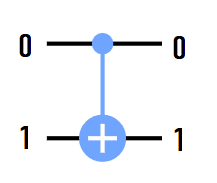
\includegraphics[scale=1]{cnot_example_1}
    \centering
\end{figure}

\begin{figure}[H]
    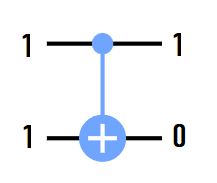
\includegraphics[scale=1]{cnot_example_2}
    \centering
\end{figure}

\par Je možné poskládat matici pro libovolné kontrolní hradlo. Ukážu to na přikladu CNOTu.
$$CNOT = |1 \rangle\langle 1| \otimes X + |0 \rangle\langle 0| \otimes I$$
$$CNOT = \begin{bmatrix}
        0 \\
        1
    \end{bmatrix}\begin{bmatrix}
        0 & 1
    \end{bmatrix} \otimes \begin{bmatrix}
        0 & 1 \\
        1 & 0
    \end{bmatrix} + \begin{bmatrix}
        1 \\
        0
    \end{bmatrix}\begin{bmatrix}
        1 & 0
    \end{bmatrix} \otimes \begin{bmatrix}
        1 & 0 \\
        0 & 1
    \end{bmatrix}$$
$$CNOT = \begin{bmatrix}
        0 & 0 & 0 & 0 \\
        0 & 0 & 0 & 0 \\
        0 & 0 & 0 & 1 \\
        0 & 0 & 1 & 0
    \end{bmatrix} + \begin{bmatrix}
        1 & 0 & 0 & 0 \\
        0 & 1 & 0 & 0 \\
        0 & 0 & 0 & 0 \\
        0 & 0 & 0 & 0
    \end{bmatrix} = \begin{bmatrix}
        1 & 0 & 0 & 0 \\
        0 & 1 & 0 & 0 \\
        0 & 0 & 0 & 1 \\
        0 & 0 & 1 & 0
    \end{bmatrix}$$

\par Stejně jako každý logický obvod lze složit z hradel AND a NOT, lze každý kvantový obvod libovolně aproximovat pouze pomocí hradel CNOT a Hadamard.
\par Zajímavým hradlem je Toffoli gate.
Může se značit jako CCNOT.
Má totiž 2 kontrolní qubity a 1 cílový.
Zde dochází k invertovaní cílového qubitu v případě že oba kontrolní jsou ve stavu 1:

$$\begin{bmatrix}
        1 & 0 & 0 & 0 & 0 & 0 & 0 & 0 \\
        0 & 1 & 0 & 0 & 0 & 0 & 0 & 0 \\
        0 & 0 & 1 & 0 & 0 & 0 & 0 & 0 \\
        0 & 0 & 0 & 1 & 0 & 0 & 0 & 0 \\
        0 & 0 & 0 & 0 & 1 & 0 & 0 & 0 \\
        0 & 0 & 0 & 0 & 0 & 1 & 0 & 0 \\
        0 & 0 & 0 & 0 & 0 & 0 & 0 & 1 \\
        0 & 0 & 0 & 0 & 0 & 0 & 1 & 0 \\
    \end{bmatrix}$$

\begin{figure}[H]
    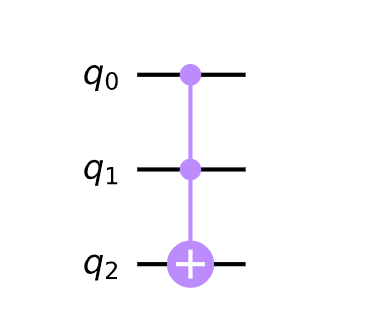
\includegraphics[scale=.7]{toffoli_scheme}
    \centering
\end{figure}

\subsection{Vzájemně spoutané qubity – Bellův Stav}
Myslím si, že je dost jasné, jak se budou chovat 2 qubity po CNOTu.
Control qubit zůstane stejný ale druhy(target) qubit se změní, pokud je první ve stavu 1.
Co se však stane, když kontrolni qubit bude v superpozici? Pojďme si to spočítat.
Budeme mít tenhle počáteční stav:
$$|\varphi_1 \rangle = |00\rangle = \begin{bmatrix}
        1 \\
        0 \\
        0 \\
        0
    \end{bmatrix}$$
\par Proto abychom dostali stav superpozice, potřebujeme hradlo Hadamarda.
V našem případě bude první qubit kontrolní, takže potřebujeme aplikovat Hadamarda na první qubit:
$$|\varphi_2 \rangle = (H \otimes I) |\varphi_1 \rangle = \frac{1}{\sqrt{2}} \begin{bmatrix}
        1 & 0 & 1  & 0  \\
        0 & 1 & 0  & 1  \\
        1 & 0 & -1 & 0  \\
        0 & 1 & 0  & -1
    \end{bmatrix}\begin{bmatrix}
        1 \\
        0 \\
        0 \\
        0
    \end{bmatrix} = \frac{1}{\sqrt{2}}\begin{bmatrix}
        1 \\
        0 \\
        1 \\
        0
    \end{bmatrix}$$
\par Tento stav nám říká, že je možný po změřeni dostat bud $|00\rangle$ nebo $|10\rangle$ s $\frac{1}{2}$ pravděpodobnosti.
Následně pojďme aplikovat CNOT:
$$|\varphi_3 \rangle = CNOT |\varphi_2 \rangle = \frac{1}{\sqrt{2}} \begin{bmatrix}
        1 & 0 & 0 & 0 \\
        0 & 1 & 0 & 0 \\
        0 & 0 & 0 & 1 \\
        0 & 0 & 1 & 0
    \end{bmatrix}\begin{bmatrix}
        1 \\
        0 \\
        1 \\
        0
    \end{bmatrix} = \frac{1}{\sqrt{2}}\begin{bmatrix}
        1 \\
        0 \\
        0 \\
        1
    \end{bmatrix}$$
\par Tímto jsme dostali Bellův stav, při němž jsou 2 qubity společně spoutány.
Ted když provedeme měřeni, dostaneme bud $|00\rangle$ nebo $|11\rangle$ s $\frac{1}{2}$ pravděpodobnosti.
Tento stav se používá u algoritmu kvantové teleportace.
Schema:
\begin{figure}[H]
    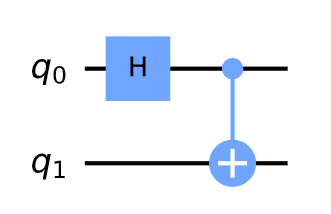
\includegraphics[scale=.7]{bell_state_scheme}
    \centering
\end{figure}

\subsection{Phase kick-back}
\label{sec:phase_kickback}
Pojďme si podívat, co se stane, pokud použijeme \textbf{X} gate na stav $|+\rangle$ nebo $|-\rangle$:
$$X|+\rangle = \frac{1}{\sqrt{2}}\begin{bmatrix}
        0 & 1 \\
        1 & 0
    \end{bmatrix} \begin{bmatrix}
        1 \\
        1
    \end{bmatrix} = \frac{1}{\sqrt{2}} \begin{bmatrix}
        1 \\
        1
    \end{bmatrix} $$

\begin{equation*}
    \begin{split}
        X|-\rangle & = \frac{1}{\sqrt{2}}\begin{bmatrix}
            0 & 1 \\
            1 & 0
        \end{bmatrix} \begin{bmatrix}
            1 \\
            -1
        \end{bmatrix} \\
        & = \frac{1}{\sqrt{2}} \begin{bmatrix}
            -1 \\
            1
        \end{bmatrix}\\
        & =  -\frac{1}{\sqrt{2}} \begin{bmatrix}
            1 \\
            -1
        \end{bmatrix}
    \end{split}
\end{equation*}
\par Na první pohled nic moc překvapivého.
Ale jedna se o první krok k porozumění důležitého konceptu: phase kick-back.
Dřive jsme si mysleli, že při použití CNOTu, ovlivňujme pouze cílový qubit.
Ale teď si úkazem, že ovlivňujme i kontrolní.
Pro demonstraci je potřeba CNOT aplikovat na cílový qubit ve stavu superpozice.
Nejdřív pro kontrolní qubit ve stavu $|0\rangle$, následně ve stavu $|1\rangle$:
$$CNOT |0-\rangle = |0\rangle \left(\frac{|0\rangle - |1\rangle}{\sqrt{2}}\right)$$
\begin{equation*}
    \begin{split}
        CNOT |1-\rangle & = |1\rangle \left(X \left(\frac{|0\rangle - |1\rangle}{\sqrt{2}}\right)\right) \\
        & = |1\rangle \left(-1\left(\frac{|0\rangle - |1\rangle}{\sqrt{2}}\right)\right) \\
        & = -|1\rangle \left(\frac{|0\rangle - |1\rangle}{\sqrt{2}}\right)
    \end{split}
\end{equation*}
\par Obecně platí:
$$CNOT |b-\rangle = (-1)^b|b\rangle\left(\frac{|0\rangle - |1\rangle}{\sqrt{2}}\right)$$:
\par Zde je vidět, že jsme dokázali změnit fázi kontrolního qubitu, když kontrolní qubit je v superpozici:
$$CNOT\left((\alpha|0\rangle + \beta|1\rangle)\left(\frac{|0\rangle - |1\rangle}{\sqrt{2}}\right)\right) = (\alpha|0\rangle - \beta|1\rangle)\left(\frac{|0\rangle - |1\rangle}{\sqrt{2}}\right)$$

\subsection{QFT a inverzní QFT}
\label{sec:qft}
Informace pro tuto kapitolu jsem čerpal hlavně z učebnice\footnote{\url{http://mmrc.amss.cas.cn/tlb/201702/W020170224608149125645.pdf}}.
\par Hadamard hradlo má ještě jednu vlastnost: můžeme pomoci nej zakódovat informaci do fáze qubitu a také ji dekódovat.
Jednoduchý příklad zakódovaní($x\in\{0,1\}$):
$$H|x\rangle = \frac{1}{\sqrt{2}}|0\rangle + \frac{(-1)^x}{\sqrt{2}}|1\rangle = \frac{1}{\sqrt{2}}\displaystyle\sum_{y\in\{0, 1\}} (-1)^{xy}|y\rangle$$
\par Pro dekódovaní aplikujme zase Hadamardovo hradlo:
$$H\left(\frac{1}{\sqrt{2}}|0\rangle + \frac{(-1)^x}{\sqrt{2}}|1\rangle\right) = |x\rangle$$
\par Obecně fázi můžeme zapsat jako komplexní číslo $e^{2\pi i w}$, kde $w\in(0, 1)$ a je reálné.
Z obrázku\footnote{\url{https://en.wikipedia.org/wiki/Euler's_formula}}, který znázorňuje geometricky smysl Eulerové rovnice,
můžeme vidět, že hodnota $\varphi$ v $e^{i\varphi}$ odpovídá úhlu otočeni bodu $[1, 0]$ kolem středu jednotkové kružnice v radiánech.
V našem případě je $\varphi = 2\pi w$.

\begin{figure}[H]
    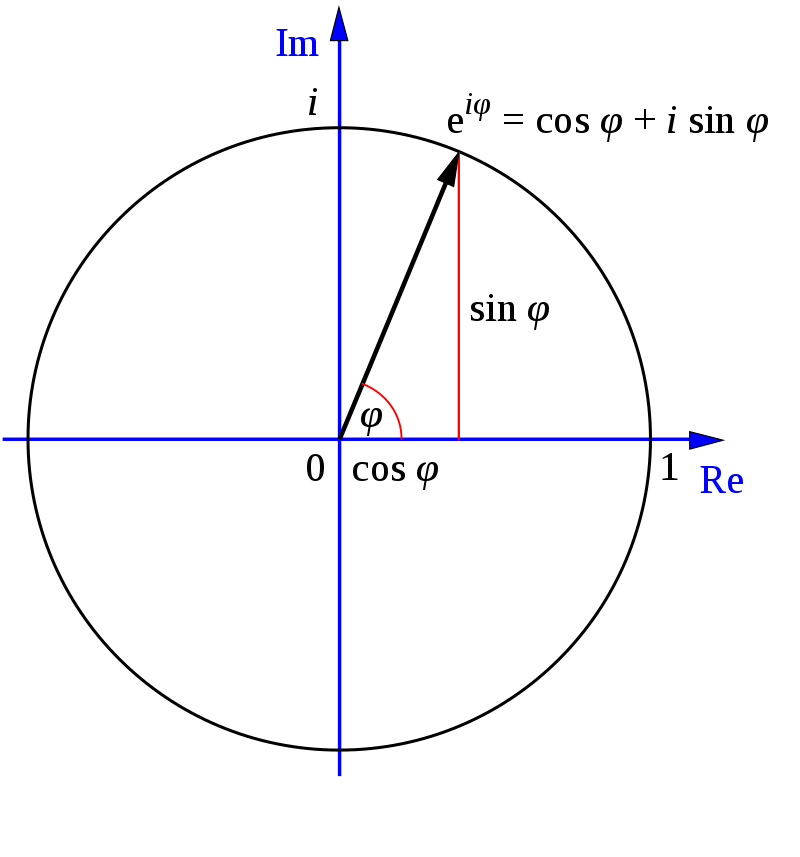
\includegraphics[scale=.25]{Eulers_formula.png}
    \centering
\end{figure}
\par Můžeme si představit $w$ jako k-bitové binární číslo $w=0.x_1x_2x_3...x_k$, to znamená $w = x_1 \cdot 2^{-1} + x_2 \cdot 2^{-2} + x_3 \cdot 2^{-3} + ... + x_k \cdot 2^{-k}$.
Pro příklad si představíme, že máme jeden qubit, pro které platí, že $w=0.x_1$.
Pak:
$$
    \frac{1}{\sqrt{2}}\displaystyle\sum_{y\in\{0, 1\}} e^{2\pi i (0.x_1) y}|y\rangle =
    \frac{1}{\sqrt{2}}\displaystyle\sum_{y\in\{0, 1\}} e^{2\pi i (\frac{x_1}{2}) y}|y\rangle =
    \frac{1}{\sqrt{2}}\displaystyle\sum_{y\in\{0, 1\}} (-1)^{xy}|y\rangle
$$
\par Tento stav můžeme dekódovat pomoci hradla Hadamarda, a tím získáme $w$.
Co když se bude $w$ skládat z $n$ bitu po desetinné čárce?
Můžeme tento komplikovaný stav rozepsat dle rovnice z učebnice\footnote{rovnice 7.1.18, \url{http://mmrc.amss.cas.cn/tlb/201702/W020170224608149125645.pdf}}.
V našem případě $w=0.x_1x_2$ a $n=2$:

$$
    \frac{1}{\sqrt{2^2}}\displaystyle\sum_{y=0}^{2^2 - 1} e^{2\pi i (0.x_1x_2) y}|y\rangle =
    \left(\frac{|0\rangle + e^{2\pi i (0.x_2)}|1\rangle}{\sqrt{2}}\right) \otimes
    \left(\frac{|0\rangle + e^{2\pi i (0.x_1x_2)}|1\rangle}{\sqrt{2}}\right)
$$

\par Všimneme si, že pro získaní $x_2$ stačí aplikovat hradlo Hadamarda na první qubit.
Dostat $x_1$ bude o něco složitější.
Proto si nadefinuji hradlo $R_k$, které mění fázi qubitu:
$$
    \begin{bmatrix}
        1 & 0                       \\
        0 & e^{\frac{2 \pi i}{2^k}}
    \end{bmatrix}
$$
inverzní hradlo $R_k^{-1}$ je:
$$
    \begin{bmatrix}
        1 & 0                        \\
        0 & e^{-\frac{2 \pi i}{2^k}}
    \end{bmatrix}
$$
\par Když je $x_2 = 1$ a hradlo $R_2^{-1}$ aplikuju na druhy qubit, dostanu následující:
$$
    R_2^{-1}\left(\frac{|0\rangle + e^{2\pi i (0.x_1 1)}|1\rangle}{\sqrt{2}}\right) =
    \frac{|0\rangle + e^{2\pi i (0.x_1 1 - 0.01)}|1\rangle}{\sqrt{2}} =
    \frac{|0\rangle + e^{2\pi i (0.x_1)}|1\rangle}{\sqrt{2}}
$$
\par Ted už jen zbývá aplikovat $H$ pro získaní $x_1$.
Všimneme si, že je potřeba aplikovat $R_k^{-1}$ pouze když je $x_{k} = 1$.
Takže je z toho potřeba vyrobit Controlled gate.
Schéma pro 2 qubity by vypadala takto\footnote{obrázek 7.1, \url{http://mmrc.amss.cas.cn/tlb/201702/W020170224608149125645.pdf}}.
\begin{figure}[H]
    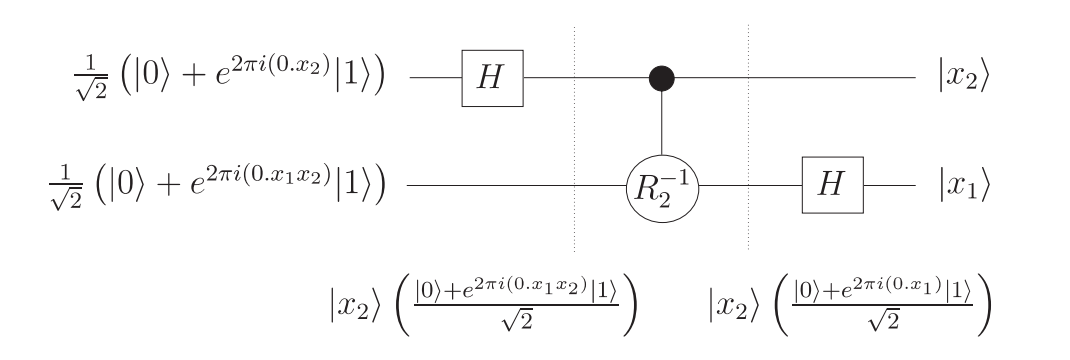
\includegraphics[scale=.6]{phase_estimation}
    \centering
\end{figure}
\par Tento proces se da zapsat jako:
$$\frac{1}{\sqrt{2^n}}\displaystyle\sum_{y=0}^{2^n - 1} e^{2\pi i \frac{x}{2^n} y}|y\rangle \to |x\rangle$$
\par Obraceny proces se označuje jako $QFT$(Quantum Fourier Transform):
$$QFT:|x\rangle \to \frac{1}{\sqrt{2^n}}\displaystyle\sum_{y=0}^{2^n - 1} e^{2\pi i \frac{x}{2^n} y}|y\rangle$$
\par Potom $QFT^{-1}$ se zapisuje:
$$QFT^{-1}:|x\rangle \to \frac{1}{\sqrt{2^n}}\displaystyle\sum_{y=0}^{2^n - 1} e^{-2\pi i \frac{x}{2^n} y}|y\rangle$$

\newpage

\section{QuantumEmulator – vlastní kvantový simulátor}
\label{sec:QuantumEmulator}
\subsection{Úvod}
QuantumEmulator – je moje vlastní Python knihovna, při jejíž implementaci jsem měl možnost do hloubky pochopit matematický model kvantových výpočtů.
Nabízí funkce pro tvorbu kvantových algoritmu libovolné složitosti.
\par Jelikož simulace kvantového počítače je hodně o počítaní s maticemi, vybral jsem si knihovnu Numpy, která zjednodušuje prací s maticemi a celkově výpočty.
Numpy využívá funkce psané v jazyce C, a proto jsou výpočty optimalizované a rychlé.
\par Projekt je pod licenci MIT a lze ho najit na mem githubu\footnote{\url{https://github.com/DimaLeshchinskiy/QuantumEmulator}}.

\subsection{QConstants}
Tento soubor obsahuje předem definované matice pro nejpoužívanější hradla a taky konstanty.
\subsection{QCircuit}
Tento soubor definuje třídu QCircuit, která obsahuje metody pro tvorbu kvantových algoritmu.
Nejdřív jsou definované funkce pro tvorbu.
\begin{itemize}
    \item \textbf{addQubits(initValues:array<int>)} - definuje počáteční stav kvantového počítače.
          Na vstup dostava seznam z 0 a 1.
    \item \textbf{addGate(gate:numpy.matrix, index:int)} - přidává hradlo pro jeden qubit se zadaným indexem.
          Pro okolní qubity se používá hradlo \textbf{I}
          Na vstup dostava matici hradla definovanou pomoci Numpy a číselný index, který odpovídá indexu qubitu z počátečního stavu.
    \item \textbf{addGates(gates:array<numpy.matrix>)} - přidává hradla pro celou skupinu qubitu.
          Na vstup dostava seznam z Numpy matic.
    \item \textbf{addControlGate(controlIndexes:array<int>, targetIndex:int, gate:numpy.matrix)} - přidává Control gate.
          Na vstup dostava seznam indexu qubitu, které budou hradlo ovládat, index cílového qubitu a Numpy matici jako matici hradla.
    \item \textbf{addCustomMatrix(matrix:numpy.matrix)} - přidává vlastní matici do obvodu.
          Na vstup dostava Numpy matici, která bude aplikovaná na všechny qubity naraz.
    \item \textbf{addCNOT(controlIndex:int, targetIndex:int)} - přidává CNOT do obvodu.
          Na vstup dostava index kontrolního qubitu a index cílového qubitu.
    \item \textbf{addToffoli(controlIndexes:array<int>, targetIndex:int)} - přidává Toffoli hradlo do obvodu.
          Na vstup dostava seznam indexu qubitu, které budou hradlo ovládat a index cílového qubitu.
    \item \textbf{addSwap(index1:int, index2:int)} - přidává Swap hradlo do obvodu.
          Na vstup dostava dva indexy qubitu, jejichž stavy budou prohozeny.
\end{itemize}
\par Dále jsou definované funkce pro spuštěni kvantové simulace.
Tyto funkce by se měli pouštět až potom co se cely algoritmus poskládá pomoci tvořících funkci:
\begin{itemize}
    \item \textbf{simulate()} - provádí sčítaní všech matic do jedné, v tom pořadí v jakém byly zadaný do algoritmu.
    \item \textbf{measure()} - provádí měřeni stavu kvantového počítače na konci simulace.
          Tato funkce se má pouštět po dokončeni funkce \textbf{simulate()}.
          Nejdřív si poskládá všechny kombinace možných stavu po měřeni a následně si pro ne dopočítá pravděpodobnost výskytu.
          Na konci náhodně dle pravděpodobnosti vybere jednu z kombinaci a tu vrátí.
    \item \textbf{measureAll(indexes:array<int>)} - provádí měřeni stavu kvantového počítače na konci simulace.
          Dostava seznam indexu qubitu pro měřeni.
          Budou změřeny pouze uvedené qubity, ostatní se ignoruji.
          Když je vstupní seznam prázdny, provádí se měřeni pro všechny qubity.
          Tato funkce se má pouštět po dokončeni funkce \textbf{simulate()}.
          Nejdřív si poskládá všechny kombinace možných stavu po měřeni a následně si pro ne dopočítá pravděpodobnost výskytu.
          Vráti všechny možné stavy a jejich pravděpodobnosti.
\end{itemize}
\subsection{QColumn}
Tento soubor definuje nápomocnou třídu QColumn, která reprezentuje jeden sloupec v zápisu kvantového algoritmu.
Má jen 2 funkce:
\begin{itemize}
    \item \textbf{set(values:array<numpy.matrix>)} - počítá matici pro sloupec.
          Na vstup dostava seznam Numpy matic, které definuji hradla.
    \item \textbf{setControl(controlIndexes:array<int>, targetIndex:int, gate: numpy.matrix)} - počítá matici pro hradlo, které bude ovládáno jedním nebo vice kontrolními qubity.
          Na vstup dostava seznam indexu qubitu, které budou hradlo ovládat, index cílového qubitu a Numpy matici hradla.
\end{itemize}

\subsection{Utility}
Složka util obsahuje nápomocné funkce, které buď využívám primo v hlavních třídách emulátoru nebo byli potřebné pro moje experimenty s kvantovými algoritmy.
\begin{itemize}
    \item \textbf{int2bin.py} - obsahuje funkce pro převod mezi desítkovou soustavou a soustavou binární.
    \item \textbf{anf.py} - obsahuje funkce pro výpočet ANF pro libovolnou funkci.
          Bylo využito pro vytvořeni blackboxu pro Deutsch–Jozsa algoritmus.
\end{itemize}

\newpage

\section{Ukázky kódu}
V téhle kapitole ukážu názorné příklady využiti mé knihovny.
Všechny tyhle ukázky jsou v souboru \textbf{example.py}.

\subsection{Dvě hradla Hadamarda za sebou}
Tenhle kód simuluje jednoduchý obvod, ve kterém se za sebou skládá 2 krát hradlo Hadamarda.
Po aplikaci dvou stejných hradel, se stav kvantového počítače nezmění, což je vidět z ukázky.
\begin{lstlisting}[language=Python, caption=Double Hadamard gates]
from qsim.qcircuit import QCircuit
from qsim.qconstants import H
circuit = QCircuit()

circuit.addQubits(0) # create 1 qubits with init value 0
circuit.addGate(H, 0) # add 1 column of gates
circuit.addGate(H, 0) # add 2 column of gates

circuit.simulate() # make calculations
state = circuit.measure() # get state of all qubits
print("#EXAMPLE 1", state) # in this case output will always be 0
\end{lstlisting}
\begin{figure}[H]
    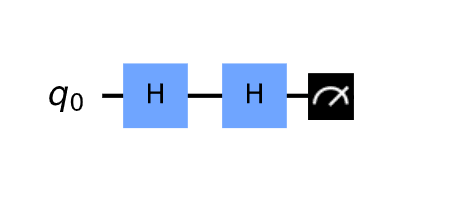
\includegraphics[scale=.5]{two_h_gates_scheme}
    \centering
\end{figure}

\subsection{Hradlo X}
Tenhle kód simuluje jednoduchý obvod, který názorně ukazuje chovaní hradla X.
\begin{lstlisting}[language=Python, caption=X gates]
from qsim.qcircuit import QCircuit
from qsim.qconstants import X
circuit = QCircuit()

circuit.addQubits(0, 0) # create 2 qubits with init value 0
circuit.addGate(X, 1) # add 1 column of gates
circuit.addGates([X, X]) # add 2 column of gates

circuit.simulate() # make calculations
state = circuit.measure() # get state of all qubits
print("#EXAMPLE 2", state) # in this case output will always be [1, 0]
\end{lstlisting}
\begin{figure}[H]
    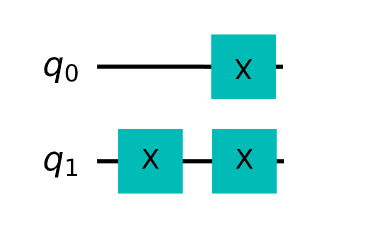
\includegraphics[scale=.5]{multiple_qubits_scheme}
    \centering
\end{figure}

\subsection{CNOT ukazka}
Tenhle kód ukazuje, jak se využívá hradlo CNOT.
\begin{lstlisting}[language=Python, caption=CNOT example]
from qsim.qcircuit import QCircuit
circuit = QCircuit()

circuit.addQubits(1, 0, 0) # create 1 qubit with init value 1 and 2 qubits with init value 0
circuit.addCNOT(controlIndex=0, targetIndex=2) # add CNOT gate with 0 index qubit as control and 2 index as target

circuit.simulate() # make calculations
state = circuit.measure() # get state of all qubits
print("#EXAMPLE 3", state) # in this case output will always be [1, 0, 1]
\end{lstlisting}
\begin{figure}[H]
    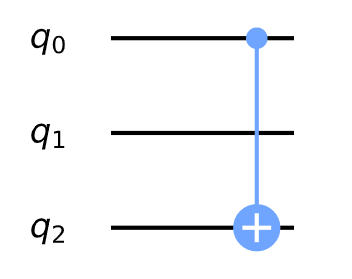
\includegraphics[scale=.5]{cnot_scheme}
    \centering
\end{figure}

\subsection{Bellův stav}
Tenhle kód ukazuje, jak lze vytvořit Bellův stav.
\begin{lstlisting}[language=Python, caption=Bell state]
from qsim.qcircuit import QCircuit
from qsim.qconstants import H, I
circuit = QCircuit()

circuit.addQubits(0, 0) # create 2 qubits with init value 0
circuit.addGates([H, I])  # add 1 column of gates
circuit.addCNOT(controlIndex=0, targetIndex=1) # add CNOT gate with 0 index qubit as control and 1 index as target

circuit.simulate() # make calculations
state = circuit.measure() # get state of all qubits
print("#EXAMPLE 4", circuit.measureAll()) # get all posible states
print("#EXAMPLE 4", state) # in this case output will be [0, 0] or [1, 1] with probability of 0.5
\end{lstlisting}
\begin{figure}[H]
    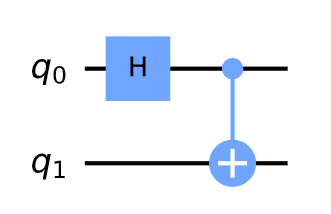
\includegraphics[scale=.5]{bell_state_scheme}
    \centering
\end{figure}

\subsection{Toffoli hradlo}
Tenhle kód ukazuje, jak lze vytvořit Toffoli hradlo.
\begin{lstlisting}[language=Python, caption=Toffoli gate]
from qsim.qcircuit import QCircuit
circuit = QCircuit()

circuit.addQubits(1, 1, 1) # create 3 qubits with init value 1
circuit.addToffoli([0, 1], 2) # add Toffole gate with 0, 1 qubits as control and 2 qubit as target

circuit.simulate() # make calculations
state = circuit.measure() # get state of all qubits
print("#EXAMPLE 5", state) # in this case output will always be [1, 1, 0]
\end{lstlisting}
\begin{figure}[H]
    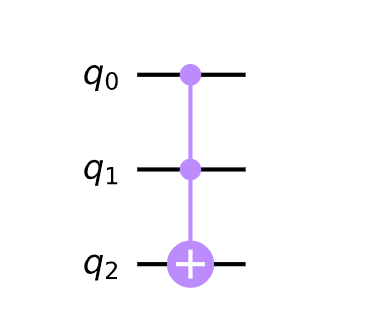
\includegraphics[scale=.7]{toffoli_scheme}
    \centering
\end{figure}

\subsection{Swap hradlo}
Tenhle kód ukazuje, jak lze vytvořit Swap hradlo.
\begin{lstlisting}[language=Python, caption=Swap gate]
from qsim.qcircuit import QCircuit
from qsim.qconstants import H, I
circuit = QCircuit()

circuit.addQubits(0, 1, 0) # create 3 qubits with init values 0, 1, 0
circuit.addGates([H, I, I])  # add 1 column of gates; create states |+10>
circuit.addSwap(0, 2) # swap qubits

circuit.simulate() # make calculations
state = circuit.measureAll() # get all posible states
print("#EXAMPLE 6", state)
\end{lstlisting}
\begin{figure}[H]
    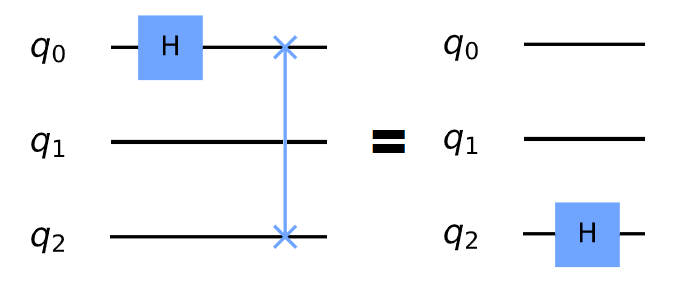
\includegraphics[scale=.7]{swap_scheme}
    \centering
\end{figure}

\newpage

\section{Shorův algoritmus}
\subsection{Úvod}
Profesor matematiky, P. Shor, přisel\footnote{\url{https://arxiv.org/pdf/quant-ph/9508027.pdf}} na to, jak rozložit K-bitové číslo na součin dvou prvočísel.
Avšak jeho algoritmus vyžaduje použít kvantové výpočty.
K tomu je potřeba přibližně $72K^3$ qubitu\footnote{\url{https://journals.aps.org/pra/abstract/10.1103/PhysRevA.54.1034}}.
Zjistil, že pro rozloženi čísla, je potřeba najit periodu funkce $f(x) = a^x \bmod N$, kde $a, N, r \in \mathbb{N}$.
Pro a platí $a < N$ a zároveň $gcd(a, N) = 1$.
Perioda $r$ je pak nejmenší možné číslo, pro které platí:
$$a^r \bmod N = 1$$
\par Proměnná $a$ se vybere náhodně z rozsahu $1 < a < N$.
Když $gcd(a, N) \ne 1$, pak jedním že součinitelů čísla $N$ je jejich nevětší společný dělitel.
Druhy lze nalézt pomoci děleni. Jinak se musí hledat perioda.
\par Problém nalezeni periody, je velice známy ve světě kvantových algoritmu.
Tento algoritmus popišu v další sekci.
\par Když periodu najdeme, zbývá jen dopočítat činitele čísla $N$ za pomocí Euklidova algoritmu pro nalezeni největšího společného dělitele.
Jelikož:
$$a^r \bmod N = 1$$
proto:
$$(a^r - 1) \bmod N = 0$$
když je $r$ sude, použijme vzorec pro rozdíl druhých mocnin:
$$a^r - 1 = (a^\frac{r}{2} + 1)(a^\frac{r}{2} - 1)$$
$$p, q = gcd(a^\frac{r}{2} \pm 1, N)$$
jinak se musí hledat $r$ dalé.

\subsection{Nalezeni periody funkce}
Pro nalezeni periody se využívá Quantum Phase Estimation algoritmus.
Jeho schéma\footnote{\sloppy\url{https://www.researchgate.net/publication/228102587_Fast_Quantum_Modular_Exponentiation_Architecture_for_Shor's_Factorization_Algorithm}}:
\begin{figure}[H]
    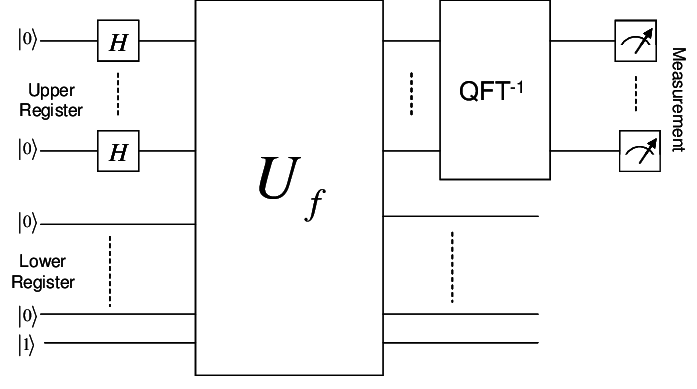
\includegraphics[scale=.5]{High-level-diagram-of-Shors-algorithm-Upper-register-consists-of-2n-qubits-and-holds}
    \centering
\end{figure}
\par Je potřeba si vytvořit dva registry. První registr pojmenuji jako kontrolní. Druhy jako cílový.
Na velikost kontrolního registru záleží to, jak moc bude velká úspěšnost dostat správný výsledek a také jak moc přesné výpočty budou.
Velikost cílového registru zvolíme jako $n = log_2(N)$.
Pak velikost $2n$ bude dostačující pro kontrolní registr.
\par Všechny qubity z kontrolního registru dáme do stavu $0$. Všechny qubity z cílového registru dáme do stavu $0$ až na poslední qubit. Ten bude ve stavu 1.
Označím je jako velké $|\textbf{0}\rangle$ a velké $|\textbf{1}\rangle$
Takže po inicializaci bude stav kvantového počítače:
$$|\varphi_1\rangle = |\textbf{0}\rangle\otimes|\textbf{1}\rangle$$
\par Dalším krokem je potřeba dostat kontrolní registr do superpozice pomoci Hadamard hradel:
$$|\varphi_2\rangle = (H^{\otimes 2n}\otimes I^{\otimes n})(|\textbf{0}\rangle\otimes|\textbf{1}\rangle)$$
\par Ted je potřeba říct, co je Uf. Toto hradlo aplikuje funkci $f(x)$ na cílový registr.
Tim, že je kontrolní registr v superpozici, dochází k \hyperref[sec:phase_kickback]{phase kick-back} jevu.
Proto zároveň při aplikaci Uf se zakóduje do fázi qubitu kontrolního registru potřebná informace.
$$Uf|x\rangle|y\rangle = |x\rangle|y \cdot f(x)\rangle = |x\rangle|ya^x \bmod N \rangle$$
\par Posledním krokem je $QFT^{-1}$.
Jedna se o inverzní hradlo k hradlu \hyperref[sec:qft]{QFT}.
QFT provádí diskretní Fourierovou transformaci\footnote{\url{https://en.wikipedia.org/wiki/Quantum_Fourier_transform}}.
$QFT^{-1}$ je potřeba pro transformaci informace z fázi kontrolních qubitu.
Ve výsledku, když změříme kontrolní registr, dostaneme číslo $x_1$.
Ted je potřeba pomoci continued fraction algoritmu, najit nejbližší zlomek ke zlomku $\frac{x_1}{2^{2n}}$, který nebude mít jmenovatel větší než $N$.
Pravě jmenovatel nalezeného zlomku je hledané $r$.
\par Tento algoritmus nemusí vždy dopočítat $r$ správně.
Proto je potřeba v praxi spustit tento algoritmus vice krát.
V našem případě použijme funkci z mé knihovny pro zisk všech kvantových stavu najednou, a proto nebude potřeba pouštět algoritmus vícekrát.

\subsection{Implementace}
Pro implementaci jsem využil svůj \hyperref[sec:QuantumEmulator]{kvantový simulátor}.
Kód lze najit na githubu v souboru shor\_example.py.
\begin{lstlisting}[language=Python, caption=Shor algorithm]
from fractions import Fraction
from math import ceil
from qsim.qcircuit import QCircuit
from qsim.qconstants import H, I, P
from qsim.util.int2bin import binToInt
import random

from numpy import log2, pi, zeros

# Euclidean algorithm
def gcd(m, n):
    if m < n: 
        (m, n) = (n, m)
    if(m % n) == 0:
        return n 
    else:
        return (gcd(n, m % n))

# return controlled phaseGate inverse R
def controlled_phaseGate_inverse(m):
    return P(-(2 * pi) / (2 ** m))

def QFT_inverse(circuit, n):
    phaseGates = [controlled_phaseGate_inverse(i) for i in range(2, n + 1)]

    for i in range(n // 2):
        circuit.addSwap(i, n - i - 1)

    for i in range(n, 0, -1):
        for phaseGateIndex in range(n - i, 0, -1):
            circuit.addControlGate(i - 1, phaseGateIndex + i - 1, phaseGates[phaseGateIndex - 1])

        circuit.addGate(H, i - 1)

def Uf(circuit, a, N):
    n1 = 2 * ceil(log2(N)) # first register size
    n2 = ceil(log2(N)) # second register size
    matrix = zeros((2 ** circuit.qbits_size, 2 ** circuit.qbits_size)) # fill matrix with zeros

    for i in range(2 ** circuit.qbits_size):
        x = i >> n2 # high n bits
        y = i & (2 ** n2 - 1) # low n bits

        # let z = (x, ya^x mod N)
        # (ya^x mod N) = (y*(a^x mod N) mod N), so for better performace
        # we will calculate (a^x mod N) separatly, because exponent could be large
        z = x << n2
        if y < N:
            func = pow(base=a, exp=x, mod=N) 
            z = z | ((y * func) % N) 
        else:
            z = z | y

        # insert 1 into column_i and row_z
        matrix[i, z] = 1
    
    # insert permutation matrix to the circuit
    circuit.addCustomMatrix(matrix)

def orderFinding(a, N):
    n1 = 2 * ceil(log2(N)) # first register size
    n2 = ceil(log2(N)) # second register size
    circuit = QCircuit()

    # fill first(control) register of size n with state 0 (|000...000>)
    # fill second(target) register of size n with state 1 (|000...001>)
    # this array represents two registers
    registers = [0] * (n1 + n2)
    registers[-1] = 1
    circuit.addQubits(*registers)

    # apply QFT to the control register
    # or apply H, which has same behavior as QFT applied to |0> ^ n
    # also it has faster implementation
    gatesH = [H] * n1
    gatesI = [I] * n2
    circuit.addGates([*gatesH, *gatesI])

    # apply Uf
    Uf(circuit, a, N)

    # apply QFT_inverse to the control register
    QFT_inverse(circuit, n1)

    circuit.simulate()

    all_r = set()
    measurments = circuit.measureAll(range(8))
    for measurement in measurments:
        state, probability = measurement
        controlRegInt = binToInt(state)

        frac = Fraction(controlRegInt, 2**n1).limit_denominator(N)
        all_r.add(frac.denominator)
    
    return all_r

# https://en.wikipedia.org/wiki/Shor%27s_algorithm
def Factorization(N):
    # step 0, if N is even
    if N % 2 == 0:
        return (2, int(N / 2))

    # step 1
    checked_a = []
    while True:
        a = 0

        while True:
            a = random.randint(2, N - 1)
            if a not in checked_a:
                checked_a.append(a)
                break

        K = gcd(a, N)

        # step 2, 3
        if K != 1:
            return (K, int(N // K))
        # step 4
        else:
            all_r = orderFinding(a, N)

            # step 5, 6, 7 
            for r in all_r:
                if r % 2 == 0 and pow(base=a, exp=r, mod=N) == 1:
                    p = gcd(pow(base=a, exp=r // 2) - 1, N)
                    q = gcd(pow(base=a, exp=r // 2) + 1, N)
                    print(f"r = {r}")
                    return (p, q)

# N = 15 max
print("Factors are: ", Factorization(15))
\end{lstlisting}

\newpage

\section{Zaver}
Prvním cílem bylo naprogramovat vlastní kvantový simulátor. Povedlo se mi vytvořit funkční knihovnu pro tvorbu a simulaci kvantových algoritmu.
Jsem schopen tvořit algoritmy libovolné složitosti.
Jedině jsem limitován operační paměti obyčejného počítače.
Během programovaní, jsem musel pochopit matematiku, kterou se popisuji kvantové algoritmy.
Ne všechny potřebné obory matematiky se probírají na střední škole,
proto nebylo jednoduché pochopit části algoritmu, kde se využívá vysokoškolská matematika.
\par Druhým cílem bylo zkusit rozložit číslo na součin dvou prvočísel pomoci algoritmu Shora a následně postup popsat.
To se mi taky povedlo.
Největší číslo, které jsem schopen rozložit je 15.
Bylo na to potřeba přibližně 12.5 GB operační paměti.
\par Moje práce může sloužit jako výukový materiál pro studenty, kteří chtějí porozumět kvantovým počítačům.
\newpage

\section{Zdroje a odkazy}
\color{blue}
\fontsize{10pt}{0}
\url{https://cs.wikipedia.org/wiki/RSA}
\par\url{https://en.wikipedia.org/wiki/Shor%27s_algorithm}
\par\url{https://en.wikipedia.org/wiki/Quantum_logic_gate}
\par\url{https://arxiv.org/pdf/quant-ph/9508027.pdf}
\par\url{https://qiskit.org/}
\par\url{http://mmrc.amss.cas.cn/tlb/201702/W020170224608149125645.pdf}
\par\url{https://en.wikipedia.org/wiki/Exponentiation_by_squaring}
\par\url{https://github.com/DimaLeshchinskiy/QuantumEmulator}

\end{document}